La computación en la nube (\textit{cloud computing}) permite ubicuidad en el acceso a un conjunto de recursos compartido, como pueden ser servidores, bases de datos, contenedores, almacenamiento, servicios, etc. Estos recursos pueden ser aprovisionados o liberados con facilidad y bajo demanda, teniendo una facturación por uso y siendo accedidos a través de la red, lo que da lugar a que esta tendencia cada vez esté mas en auge. Los recursos ofrecidos al usuario son ilimitados, teniendo a su disposición arquitecturas de computación realmente complejas y modernas sin un coste desorbitado.\\
Antes del \textit{cloud computing} el hecho de crear un servidor que funcionase 24 horas al día, 7 días a la semana era algo costoso, ya que no solo implica la inversión de la máquina si no que conlleva unos costes de mantenimiento (alimentación y red constantes, mejora de componentes desfasados a lo largos del tiempo, mantenimiento técnico, etc). Con esta nueva tendencia, es posible contratar el servicio deseado facturando únicamente por uso sin necesidad de todos los gastos anteriores.\\

El primer paso es analizar que recursos en la nube son necesarios para la aplicación web de este \gls{TFG}. Existen un gran tipo de recursos disponibles de distintos proveedores:
\begin{itemize}
\item Instancias
\item Bases de Datos SQL
\item Bases de Datos NoSQL
\item Almacenamiento en la nube
\item IP virtuales SSL
\end{itemize}

Por un lado es interesante que la persistencia del sistema cuente con un recurso propio, para lo que sería necesario una base de datos SQL, pues se utiliza el framework SQLAlchemy que trabaja sobre bases de datos SQL. El proveedor elegido para la instancia de este recurso ha sido la plataforma \textbf{IBM Cloud}~\cite{IMB} (Figura~\ref{fig:IBMCloud}).
\begin{figure}[H]
            \centering
            
\includegraphics[width=5cm]{figs/ibm_logo.png}
            \caption{Logo de la plataforma IBM Cloud}
            \label{fig:IBMCloud}
\end{figure}

IBM Cloud combina una plataforma como servicio (\gls{PaaS}) y una infraestructura como servicio (\gls{IaaS}) poniendo a disposición de desarrolladores un catálogo de recursos muy amplio. Ha sido elegido debido a que numerosos recursos de dicho catálogo cuentan con una opción \textit{lite} con capacidades limitadas totalmente gratuita, idónea para pequeños desarrolladores que se inician en la experiencia del \textit{cloud computing}. En la Figura \ref{fig:catalogoIBM} se muestran los recursos \textit{lite} en la categoría de bases de datos que IBM cloud ofrece.
\begin{figure}[H]
            \centering
            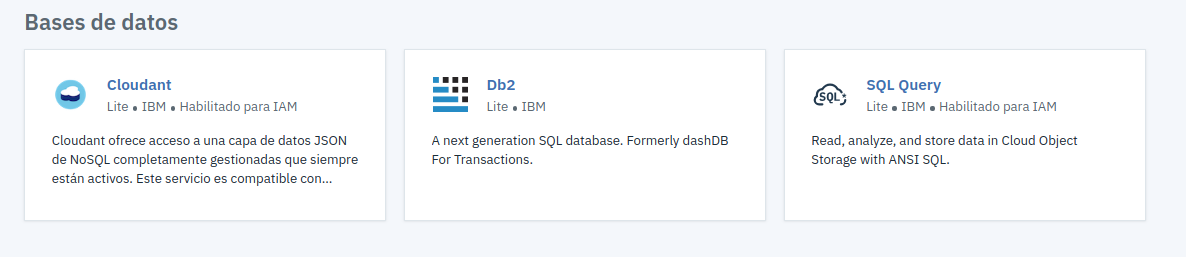
\includegraphics[width=14cm]{figs/db_ibm.png}
            \caption{Catálogo de Bases de Datos en IBM Cloud}
            \label{fig:catalogoIBM}
\end{figure}
Puesto que es necesario una base de datos SQL el recurso elegido ha sido \textbf{Db2}. Este servicio ofrece una base de datos SQL de 200 MB en su versión gratuita con copias de seguridad y permitiendo cinco conexiones simultáneas, algo más que suficiente para lo necesario en este \gls{TFG}. Una vez adquirido el recurso se permite el acceso a una consola de gestión de la base de datos que permite ver información acerca de las conexiones recibidas, información de la base de datos como tablas y registros existentes, almacenamiento restante, etc.\\El primer paso tras la obtención del recurso es generar las credenciales del servicio. Estas credenciales son proporcionadas en formato \gls{JSON} y contienen información como hostname, usuario, puerto, ssldsn, uri, etc. Para realizar la integración de esta base de datos de producción remota en la aplicación web antes debe instalarse en la máquina del servidor el controlador ibm\_db\_sa que permite las conexiones entre db2 y el framework SQLAlchemy.\\El siguiente paso es actualizar en el fichero de configuración de la aplicación Flask para producción la constante \textbf{SQLALCHEMY\_DATABASE\_URI} (listado~\ref{lst:Db2URI}) que actualmente se encuentra apuntando a una base de datos local sqlite. Su nuevo valor será el URI generado anteriormente en las credenciales del servicio. El URI es un identificador de recursos uniforme, que permite apuntar inequívocamente a la base de datos de IBM, pues contiene toda la información necesaria (usuario, key, puerto, host, etc). Cada uno de estos valores se ha añadido al fichero de constantes del proyecto (\textit{project\_constants}) excepto la contraseña, que por medida de seguridad es obtenida de las variables de entorno. Cuando la instancia de la aplicación Flask se inicia con la nueva configuración, la conexión con la base de datos de IBM se realiza y las operaciones son efectuadas en ella. Como anotación, la base de datos de test sigue siendo utilizada en local, pues no tiene sentido instanciar en la nube una base de datos con este fin ya que tras ejecutar los test es limpiada y no contiene información relevante.\\
\begin{lstlisting}[language=Python,float=ht,numbers=none,caption={URI de Db2 para SQLAlchemy en \textit{prod\_config}},label={lst:Db2URI}]
SQLALCHEMY_DATABASE_URI = 'db2://{}:{}@{}:{}/{}'.format(
                                      const.IBM_USER,
                                      os.environ['DB2_EOPTIMIZER_KEY'],
                                      const.IBM_HOSTNAME,
                                      const.IBM_PORT,
                                      const.IBM_DB
                                      )
\end{lstlisting}

Por otro lado, la aplicación web de este trabajo necesita de un servidor que ha de estar funcionando constantemente, para el cuál sería necesario una instancia. El proveedor elegido para este recurso ha sido \textbf{Amazon Web Services}~\cite{AWS} (Figura~\ref{fig:AWS}).
\begin{figure}[H]
            \centering
            
\includegraphics[width=4cm]{figs/aws_logo.png}
            \caption{Logo de Amazon Web Services}
            \label{fig:AWS}
\end{figure}

\gls{AWS} proporciona una infraestructura como servicio (\gls{IaaS}) para empresas y desarrolladores en forma de servicios web. Es una infraestructura escalable, segura, de bajo costo y muy flexible lo que lo convierte en uno de los principales proveedores en el mundo del \textit{cloud computing}. La Universidad de Castilla-La Mancha cuenta con un convenio que permite acceso a la iniciativa AWS Educate, mediante la cuál Amazon proporciona acceso a los recursos de Amazon Web Services a los estudiantes IT, entre otras ventajas.\\
De entre todos los recursos existentes en el catálogo de \gls{AWS}, para este \gls{TFG} se hará uso de una instancia \gls{EC2}, la cuál proporciona capacidad de computación escalable en la nube, eliminando la necesidad de invertir en hardware. Puesto que \gls{AWS} es una infraestructura escalable, existen numerosas configuraciones a la hora de crear una instancia \gls{EC2}. En la Tabla~\ref{tab:EC2instance} se muestra la configuración de la instancia creada para la aplicación web de este \gls{TFG}. En la Figura~\ref{fig:AWSControlPanel} se muestra el panel de control de instancias de \gls{AWS}, con la información referente a la instancia creada.
\begin{table}[hp]
        \centering
        \begin{tabular}{|l|c|}
                \hline
                Tipo de instancia & t2.micro \\ \hline
                Sistema Operativo & Ubuntu Server 18.04 LTS \\ \hline
                Memoria & 1 GB \\ \hline
                Disco & 8 GB SSD \\ \hline
             \end{tabular}
        \caption{Instancia EC2 creada en AWS}
        \label{tab:EC2instance}
\end{table}

\begin{figure}[H]
            \centering
            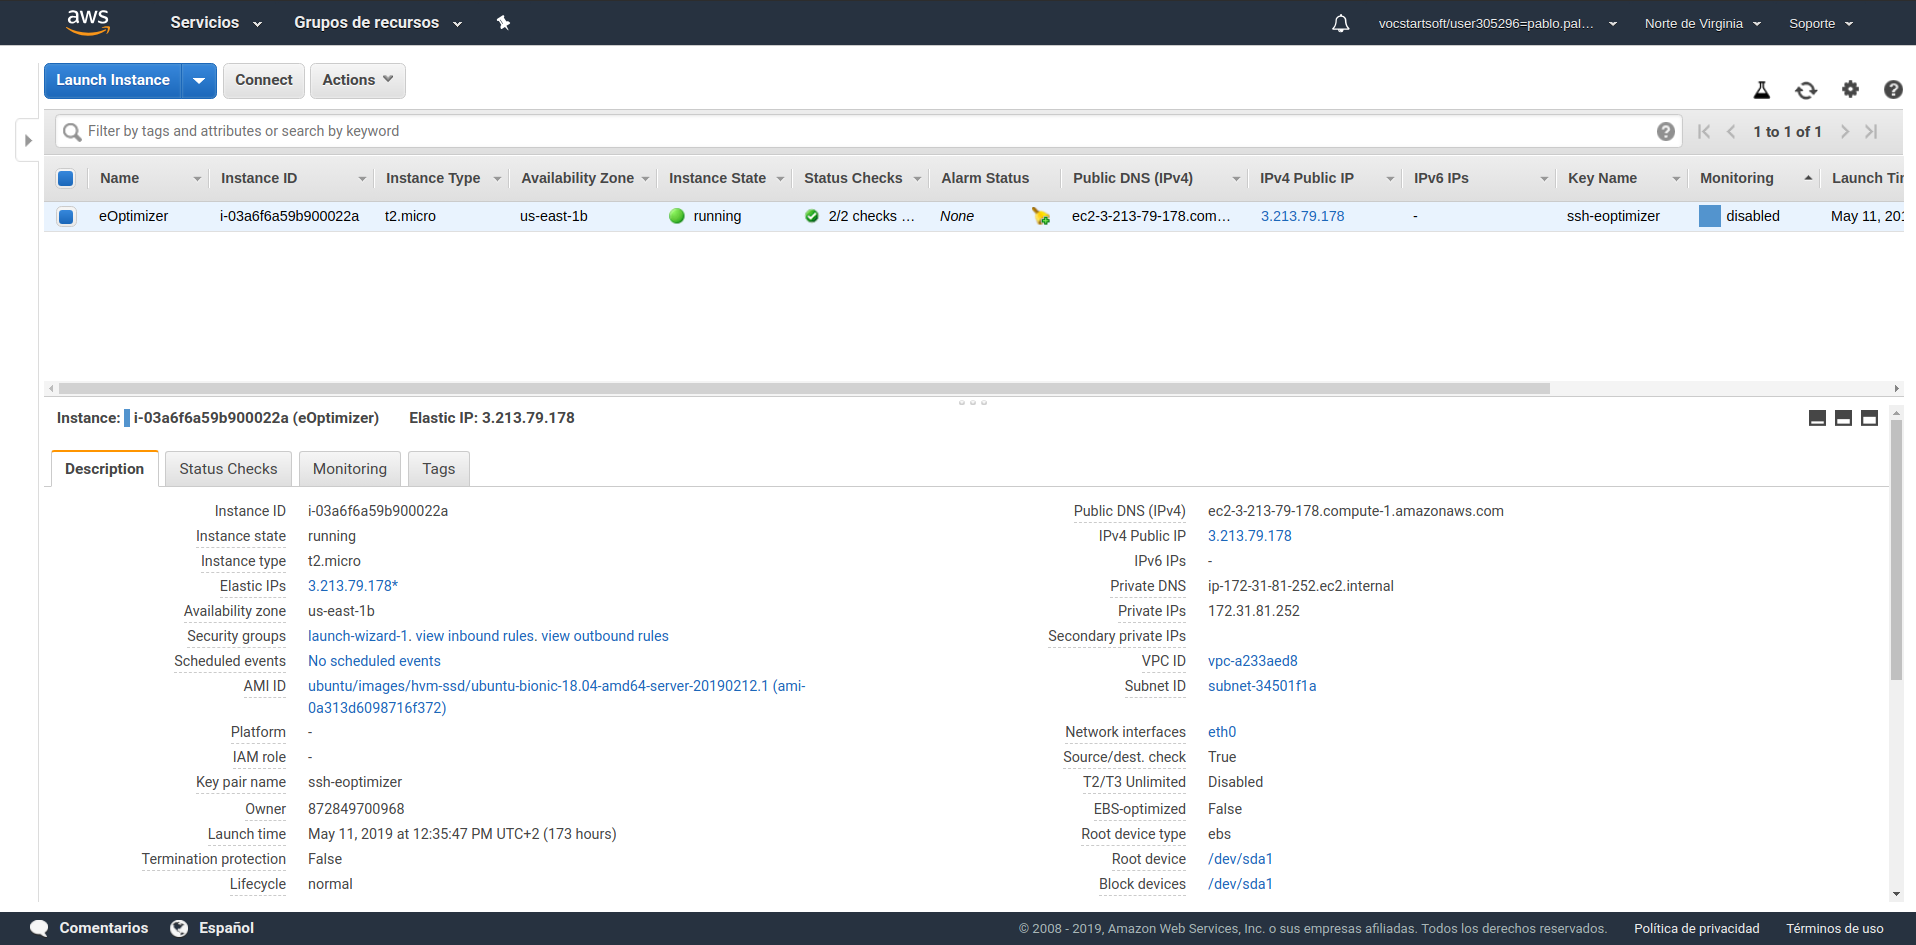
\includegraphics[width=17cm]{figs/aws_control_panel.png}
            \caption{Panel de control de instancias AWS}
            \label{fig:AWSControlPanel}
\end{figure}

Una vez seleccionada la instancia, el siguiente paso es generar la claves ssh. Esto permitirá el acceso remoto mediante el protocolo ssh a la máquina, la cuál es preparada para ejecutar la aplicación web mediante la instalación de las dependencias necesarias. Cuando el servidor esté corriendo, este será accesible a través de la IP pública de la instancia \gls{EC2} y el puerto seleccionado para la aplicación. Dicha IP es una \textbf{IP elástica} proporcionada por \gls{AWS}, las cuáles tienen la capacidad de enmascarar los errores producidos en una instacia reasignando rápidamente la dirección con otra instancia similar del usuario \gls{AWS}. Para permitir la ejecución constante de la aplicación web se han creado dos tareas \textbf{cron}. Cron es un administrador regular de procesos -demonios- que permite pogramar tareas disparadas por tiempo, fecha o procesos, permitiendo automatizar las tareas de gestión de un servidor web como ponerlo en funcionamiento, pararlo, limpiar ficheros basura generados, etc. Se ha decidido crear dos script bash, el primero para ejecutar la aplicación web y el segundo para parar su ejecución y limpiar los archivos generados (copias de los reportes de simulación realizados). Las tareas cron creadas para el mantenimiento del servidor han sido las siguientes:
\begin{itemize}
\item Cada semana la aplicación web es parada durante la madrugada, y arrancada nuevamente tras la limpieza de basura generada durante la semana.
\item Cuando la instancia \gls{EC2} se inicia, la aplicación se ejecuta. Esto es debido a posibles errores en la instancia \gls{EC2} que requieran su reinicio, permitiendo así que esto no afecte al servidor.
\end{itemize}

Tras esta iteración la aplicación web eOptimizer se encuentra en constante funcionamiento accesible mediante el socket (dirección IP y puerto) mostrado a continuación, cuyos dos recursos se encuentran alojados en la nube, cada uno en un proveedor distinto y conectados entre sí.\\

\centerline{\url{http://3.213.79.178:5000/}}
